% Options for packages loaded elsewhere
\PassOptionsToPackage{unicode=true}{hyperref}
\PassOptionsToPackage{hyphens}{url}
%
\documentclass[
]{article}
\usepackage{lmodern}
\usepackage{amssymb,amsmath}
\usepackage{ifxetex,ifluatex}
\ifnum 0\ifxetex 1\fi\ifluatex 1\fi=0 % if pdftex
  \usepackage[T1]{fontenc}
  \usepackage[utf8]{inputenc}
  \usepackage{textcomp} % provides euro and other symbols
\else % if luatex or xelatex
  \usepackage{unicode-math}
  \defaultfontfeatures{Scale=MatchLowercase}
  \defaultfontfeatures[\rmfamily]{Ligatures=TeX,Scale=1}
\fi
% Use upquote if available, for straight quotes in verbatim environments
\IfFileExists{upquote.sty}{\usepackage{upquote}}{}
\IfFileExists{microtype.sty}{% use microtype if available
  \usepackage[]{microtype}
  \UseMicrotypeSet[protrusion]{basicmath} % disable protrusion for tt fonts
}{}
\makeatletter
\@ifundefined{KOMAClassName}{% if non-KOMA class
  \IfFileExists{parskip.sty}{%
    \usepackage{parskip}
  }{% else
    \setlength{\parindent}{0pt}
    \setlength{\parskip}{6pt plus 2pt minus 1pt}}
}{% if KOMA class
  \KOMAoptions{parskip=half}}
\makeatother
\usepackage{xcolor}
\IfFileExists{xurl.sty}{\usepackage{xurl}}{} % add URL line breaks if available
\IfFileExists{bookmark.sty}{\usepackage{bookmark}}{\usepackage{hyperref}}
\hypersetup{
  pdftitle={Rasterdiv basics. Derive indices of diversity from NDVI.},
  pdfauthor={Matteo Marcantonio, Duccio Rocchini},
  hidelinks,
}
\urlstyle{same} % disable monospaced font for URLs
\usepackage[margin=1in]{geometry}
\usepackage{color}
\usepackage{fancyvrb}
\newcommand{\VerbBar}{|}
\newcommand{\VERB}{\Verb[commandchars=\\\{\}]}
\DefineVerbatimEnvironment{Highlighting}{Verbatim}{commandchars=\\\{\}}
% Add ',fontsize=\small' for more characters per line
\usepackage{framed}
\definecolor{shadecolor}{RGB}{248,248,248}
\newenvironment{Shaded}{\begin{snugshade}}{\end{snugshade}}
\newcommand{\AlertTok}[1]{\textcolor[rgb]{0.94,0.16,0.16}{#1}}
\newcommand{\AnnotationTok}[1]{\textcolor[rgb]{0.56,0.35,0.01}{\textbf{\textit{#1}}}}
\newcommand{\AttributeTok}[1]{\textcolor[rgb]{0.77,0.63,0.00}{#1}}
\newcommand{\BaseNTok}[1]{\textcolor[rgb]{0.00,0.00,0.81}{#1}}
\newcommand{\BuiltInTok}[1]{#1}
\newcommand{\CharTok}[1]{\textcolor[rgb]{0.31,0.60,0.02}{#1}}
\newcommand{\CommentTok}[1]{\textcolor[rgb]{0.56,0.35,0.01}{\textit{#1}}}
\newcommand{\CommentVarTok}[1]{\textcolor[rgb]{0.56,0.35,0.01}{\textbf{\textit{#1}}}}
\newcommand{\ConstantTok}[1]{\textcolor[rgb]{0.00,0.00,0.00}{#1}}
\newcommand{\ControlFlowTok}[1]{\textcolor[rgb]{0.13,0.29,0.53}{\textbf{#1}}}
\newcommand{\DataTypeTok}[1]{\textcolor[rgb]{0.13,0.29,0.53}{#1}}
\newcommand{\DecValTok}[1]{\textcolor[rgb]{0.00,0.00,0.81}{#1}}
\newcommand{\DocumentationTok}[1]{\textcolor[rgb]{0.56,0.35,0.01}{\textbf{\textit{#1}}}}
\newcommand{\ErrorTok}[1]{\textcolor[rgb]{0.64,0.00,0.00}{\textbf{#1}}}
\newcommand{\ExtensionTok}[1]{#1}
\newcommand{\FloatTok}[1]{\textcolor[rgb]{0.00,0.00,0.81}{#1}}
\newcommand{\FunctionTok}[1]{\textcolor[rgb]{0.00,0.00,0.00}{#1}}
\newcommand{\ImportTok}[1]{#1}
\newcommand{\InformationTok}[1]{\textcolor[rgb]{0.56,0.35,0.01}{\textbf{\textit{#1}}}}
\newcommand{\KeywordTok}[1]{\textcolor[rgb]{0.13,0.29,0.53}{\textbf{#1}}}
\newcommand{\NormalTok}[1]{#1}
\newcommand{\OperatorTok}[1]{\textcolor[rgb]{0.81,0.36,0.00}{\textbf{#1}}}
\newcommand{\OtherTok}[1]{\textcolor[rgb]{0.56,0.35,0.01}{#1}}
\newcommand{\PreprocessorTok}[1]{\textcolor[rgb]{0.56,0.35,0.01}{\textit{#1}}}
\newcommand{\RegionMarkerTok}[1]{#1}
\newcommand{\SpecialCharTok}[1]{\textcolor[rgb]{0.00,0.00,0.00}{#1}}
\newcommand{\SpecialStringTok}[1]{\textcolor[rgb]{0.31,0.60,0.02}{#1}}
\newcommand{\StringTok}[1]{\textcolor[rgb]{0.31,0.60,0.02}{#1}}
\newcommand{\VariableTok}[1]{\textcolor[rgb]{0.00,0.00,0.00}{#1}}
\newcommand{\VerbatimStringTok}[1]{\textcolor[rgb]{0.31,0.60,0.02}{#1}}
\newcommand{\WarningTok}[1]{\textcolor[rgb]{0.56,0.35,0.01}{\textbf{\textit{#1}}}}
\usepackage{graphicx,grffile}
\makeatletter
\def\maxwidth{\ifdim\Gin@nat@width>\linewidth\linewidth\else\Gin@nat@width\fi}
\def\maxheight{\ifdim\Gin@nat@height>\textheight\textheight\else\Gin@nat@height\fi}
\makeatother
% Scale images if necessary, so that they will not overflow the page
% margins by default, and it is still possible to overwrite the defaults
% using explicit options in \includegraphics[width, height, ...]{}
\setkeys{Gin}{width=\maxwidth,height=\maxheight,keepaspectratio}
\setlength{\emergencystretch}{3em} % prevent overfull lines
\providecommand{\tightlist}{%
  \setlength{\itemsep}{0pt}\setlength{\parskip}{0pt}}
\setcounter{secnumdepth}{-\maxdimen} % remove section numbering
% Redefines (sub)paragraphs to behave more like sections
\ifx\paragraph\undefined\else
  \let\oldparagraph\paragraph
  \renewcommand{\paragraph}[1]{\oldparagraph{#1}\mbox{}}
\fi
\ifx\subparagraph\undefined\else
  \let\oldsubparagraph\subparagraph
  \renewcommand{\subparagraph}[1]{\oldsubparagraph{#1}\mbox{}}
\fi

% Set default figure placement to htbp
\makeatletter
\def\fps@figure{htbp}
\makeatother


\title{Rasterdiv basics. Derive indices of diversity from NDVI.}
\author{Matteo Marcantonio, Duccio Rocchini}
\date{}

\begin{document}
\maketitle

\begin{Shaded}
\begin{Highlighting}[]
\CommentTok{#Required packages}
\KeywordTok{library}\NormalTok{(rasterdiv)}
\KeywordTok{library}\NormalTok{(rasterVis)}
\KeywordTok{library}\NormalTok{(RColorBrewer)}
\end{Highlighting}
\end{Shaded}

This vignette uses \textbf{rasterdiv} to build global series of indices
of diversity based on Information Theory. The input dataset is the
Copernicus Long-term (1999-2017) average Normalise Difference Vegetation
Index for the 21st of June (copNDVI).

\hypertarget{overview}{%
\subsection{Overview}\label{overview}}

A RasterLayer called copNDVI is loaded together with package
\textbf{rasterdiv}. \emph{copNDVI} is at 8-bit meaning that pixel values
range from 0 to 255 (you could \emph{stretch} it to a more familiar
(-1,1) range using \texttt{raster::stretch(copNDVI,minv=-1,maxv=1)}).

\hypertarget{reclassify-ndvi}{%
\subsection{Reclassify NDVI}\label{reclassify-ndvi}}

Pixels with values 253, 254 and 255 (water) will be set as NA's.

\begin{Shaded}
\begin{Highlighting}[]
\NormalTok{copNDVI <-}\StringTok{ }\KeywordTok{reclassify}\NormalTok{(copNDVI, }\KeywordTok{cbind}\NormalTok{(}\DecValTok{253}\NormalTok{, }\DecValTok{255}\NormalTok{, }\OtherTok{NA}\NormalTok{), }\DataTypeTok{right=}\OtherTok{TRUE}\NormalTok{)}
\end{Highlighting}
\end{Shaded}

\hypertarget{resample-ndvi-to-coarser-resolution}{%
\subsection{Resample NDVI to coarser
resolution}\label{resample-ndvi-to-coarser-resolution}}

To speed up the calculation, the RasterLayer will be ``resampled'' at a
resolution 20 times coarser than original.

\begin{Shaded}
\begin{Highlighting}[]
\CommentTok{#Make a raster with target resolution}
\NormalTok{rtar <-}\StringTok{ }\KeywordTok{raster}\NormalTok{(}\DataTypeTok{nrow=}\DecValTok{3920}\OperatorTok{/}\DecValTok{40}\NormalTok{,}\DataTypeTok{ncol=}\DecValTok{10080}\OperatorTok{/}\DecValTok{40}\NormalTok{,}\DataTypeTok{ext=}\KeywordTok{extent}\NormalTok{(copNDVI))}
\CommentTok{#Resample using bilinear sampling}
\NormalTok{copNDVIlr <-}\StringTok{ }\KeywordTok{resample}\NormalTok{(copNDVI, rtar, }\DataTypeTok{method =} \StringTok{"bilinear"}\NormalTok{)}
\CommentTok{#Set float numbers as integers}
\KeywordTok{storage.mode}\NormalTok{(copNDVIlr[]) =}\StringTok{ "integer"}
\end{Highlighting}
\end{Shaded}

\hypertarget{compare-ndvi-low-and-high-resolution}{%
\subsection{Compare NDVI low and high
resolution}\label{compare-ndvi-low-and-high-resolution}}

\begin{Shaded}
\begin{Highlighting}[]
\KeywordTok{levelplot}\NormalTok{(copNDVI,}\DataTypeTok{layout=}\KeywordTok{c}\NormalTok{(}\DecValTok{0}\NormalTok{,}\DecValTok{1}\NormalTok{,}\DecValTok{1}\NormalTok{), }\DataTypeTok{main=}\StringTok{"NDVI 21st of June 1999-2017 - ~5km pixel resolution"}\NormalTok{)}
\end{Highlighting}
\end{Shaded}

\begin{center}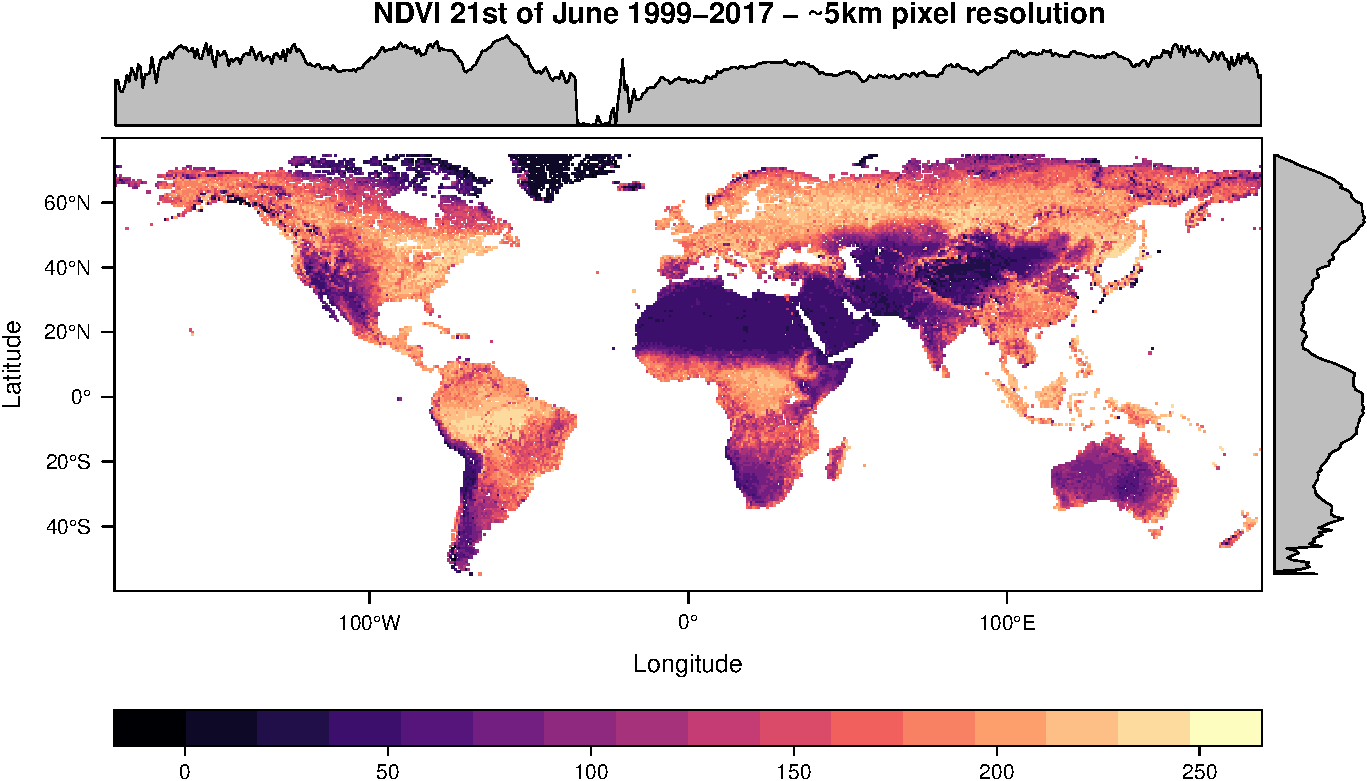
\includegraphics[width=0.95\linewidth]{vignettes_rasterdiv_files/figure-latex/fig01-1} \end{center}

\begin{Shaded}
\begin{Highlighting}[]
\KeywordTok{levelplot}\NormalTok{(copNDVIlr,}\DataTypeTok{layout=}\KeywordTok{c}\NormalTok{(}\DecValTok{0}\NormalTok{,}\DecValTok{1}\NormalTok{,}\DecValTok{1}\NormalTok{), }\DataTypeTok{main=}\StringTok{"NDVI 21st of June 1999-2017 - ~100km pixel resolution"}\NormalTok{)}
\end{Highlighting}
\end{Shaded}

\begin{center}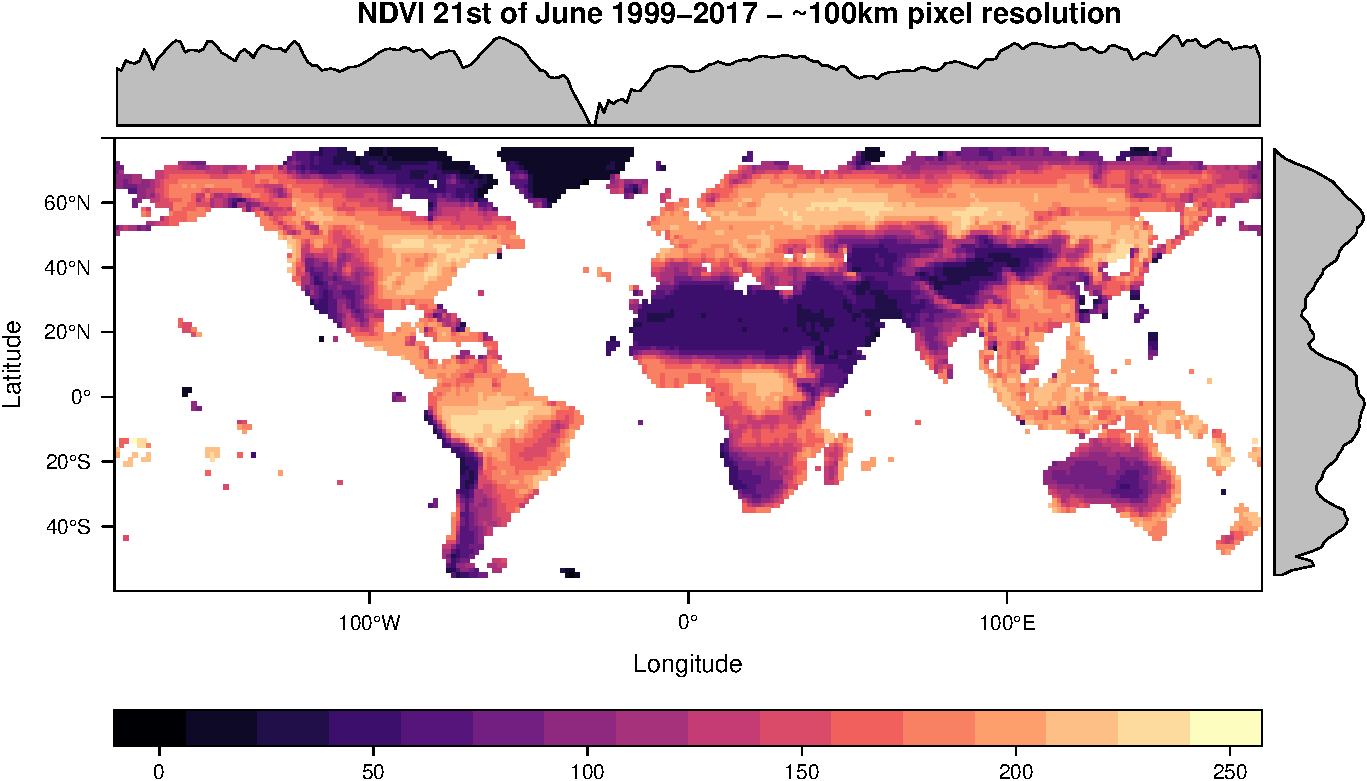
\includegraphics[width=0.95\linewidth]{vignettes_rasterdiv_files/figure-latex/fig01-2} \end{center}

\hypertarget{derive-hills-and-renyis-indices}{%
\subsection{Derive Hill's and Renyi's
indices}\label{derive-hills-and-renyis-indices}}

Renyi and Hill's indices are calculated from copNDVI with a moving
window of 81 pixels (9 px side) for alpha values from 0 to 2 every 0.5.
In addition, we set \texttt{na.tolerance=0.5}, meaning that pixels whose
9x9 px window has more than 50\% of NA values will be set to NA.

\begin{Shaded}
\begin{Highlighting}[]
\CommentTok{#Shannon's Diversity}
\NormalTok{sha <-}\StringTok{ }\KeywordTok{Shannon}\NormalTok{(copNDVIlr,}\DataTypeTok{window=}\DecValTok{9}\NormalTok{,}\DataTypeTok{np=}\DecValTok{1}\NormalTok{,}\DataTypeTok{na.tolerance=}\FloatTok{0.1}\NormalTok{)}

\CommentTok{#Pielou's Evenness}
\NormalTok{pie <-}\StringTok{ }\KeywordTok{Pielou}\NormalTok{(copNDVIlr,}\DataTypeTok{window=}\DecValTok{9}\NormalTok{,}\DataTypeTok{np=}\DecValTok{1}\NormalTok{,}\DataTypeTok{na.tolerance=}\FloatTok{0.1}\NormalTok{)}

\CommentTok{#Berger-Parker}
\NormalTok{ber <-}\StringTok{ }\KeywordTok{BergerParker}\NormalTok{(copNDVIlr,}\DataTypeTok{window=}\DecValTok{9}\NormalTok{,}\DataTypeTok{np=}\DecValTok{1}\NormalTok{,}\DataTypeTok{na.tolerance=}\FloatTok{0.1}\NormalTok{)}

\CommentTok{#Rao's quadratic Entropy}
\NormalTok{rao <-}\StringTok{ }\KeywordTok{Rao}\NormalTok{(copNDVIlr,}\DataTypeTok{window=}\DecValTok{9}\NormalTok{,}\DataTypeTok{np=}\DecValTok{1}\NormalTok{,}\DataTypeTok{na.tolerance=}\FloatTok{0.1}\NormalTok{,}\DataTypeTok{dist_m=}\StringTok{"euclidean"}\NormalTok{,}\DataTypeTok{shannon=}\OtherTok{FALSE}\NormalTok{)}

\CommentTok{#Cumulative Residual Entropy}
\NormalTok{cre <-}\StringTok{ }\KeywordTok{CRE}\NormalTok{(copNDVIlr,}\DataTypeTok{window=}\DecValTok{9}\NormalTok{,}\DataTypeTok{np=}\DecValTok{1}\NormalTok{,}\DataTypeTok{na.tolerance=}\FloatTok{0.1}\NormalTok{)}

\CommentTok{#Hill's numbers}
\NormalTok{hil <-}\StringTok{ }\KeywordTok{Hill}\NormalTok{(copNDVIlr,}\DataTypeTok{window=}\DecValTok{9}\NormalTok{,}\DataTypeTok{np=}\DecValTok{1}\NormalTok{,}\DataTypeTok{na.tolerance=}\FloatTok{0.1}\NormalTok{,}\DataTypeTok{alpha=}\KeywordTok{seq}\NormalTok{(}\DecValTok{0}\NormalTok{,}\DecValTok{2}\NormalTok{,}\FloatTok{0.5}\NormalTok{))}

\CommentTok{#Renyi}
\NormalTok{ren <-}\StringTok{ }\KeywordTok{Renyi}\NormalTok{(copNDVIlr,}\DataTypeTok{window=}\DecValTok{9}\NormalTok{,}\DataTypeTok{np=}\DecValTok{1}\NormalTok{,}\DataTypeTok{na.tolerance=}\FloatTok{0.1}\NormalTok{,}\DataTypeTok{alpha=}\KeywordTok{seq}\NormalTok{(}\DecValTok{0}\NormalTok{,}\DecValTok{2}\NormalTok{,}\FloatTok{0.5}\NormalTok{))}
\end{Highlighting}
\end{Shaded}

\hypertarget{transform-output-matrices-to-rasterlayer}{%
\subsection{Transform output matrices to
RasterLayer}\label{transform-output-matrices-to-rasterlayer}}

All functions in \emph{rasterdiv} output numerical matrices or list of
numerical matrices. Therefore, they need to be placed in space to be
transformed in RasterLayer. This is done by using the input NDVI
RasterLayer as template.

\begin{Shaded}
\begin{Highlighting}[]
\NormalTok{shara <-}\StringTok{ }\KeywordTok{raster}\NormalTok{(sha,}\DataTypeTok{template=}\NormalTok{copNDVIlr)}
\NormalTok{piera <-}\StringTok{ }\KeywordTok{raster}\NormalTok{(pie,}\DataTypeTok{template=}\NormalTok{copNDVIlr)}
\NormalTok{berra <-}\StringTok{ }\KeywordTok{raster}\NormalTok{(ber,}\DataTypeTok{template=}\NormalTok{copNDVIlr)}
\NormalTok{raora <-}\StringTok{ }\KeywordTok{raster}\NormalTok{(rao,}\DataTypeTok{template=}\NormalTok{copNDVIlr)}
\NormalTok{crera <-}\StringTok{ }\KeywordTok{raster}\NormalTok{(cre,}\DataTypeTok{template=}\NormalTok{copNDVIlr)}
\NormalTok{hilra <-}\StringTok{ }\KeywordTok{lapply}\NormalTok{(hil, }\ControlFlowTok{function}\NormalTok{(x) }\KeywordTok{raster}\NormalTok{(x,}\DataTypeTok{template=}\NormalTok{copNDVIlr))}
\NormalTok{renra <-}\StringTok{ }\KeywordTok{lapply}\NormalTok{(ren, }\ControlFlowTok{function}\NormalTok{(x) }\KeywordTok{raster}\NormalTok{(x,}\DataTypeTok{template=}\NormalTok{copNDVIlr))}
\end{Highlighting}
\end{Shaded}

\hypertarget{visualise-rasterlayers}{%
\subsection{Visualise RasterLayers}\label{visualise-rasterlayers}}

\begin{Shaded}
\begin{Highlighting}[]
\CommentTok{#Shannon's Diversity}
\KeywordTok{levelplot}\NormalTok{(shara,}\DataTypeTok{main=}\StringTok{"Shannon's entropy from Copernicus NDVI 5 km (9 px-side moving window)"}\NormalTok{,}\DataTypeTok{as.table =}\NormalTok{ T,}\DataTypeTok{layout=}\KeywordTok{c}\NormalTok{(}\DecValTok{0}\NormalTok{,}\DecValTok{1}\NormalTok{,}\DecValTok{1}\NormalTok{), }\DataTypeTok{ylim=}\KeywordTok{c}\NormalTok{(}\OperatorTok{-}\DecValTok{60}\NormalTok{,}\DecValTok{75}\NormalTok{), }\DataTypeTok{margin =} \KeywordTok{list}\NormalTok{(}\DataTypeTok{draw =} \OtherTok{TRUE}\NormalTok{))}
\end{Highlighting}
\end{Shaded}

\begin{center}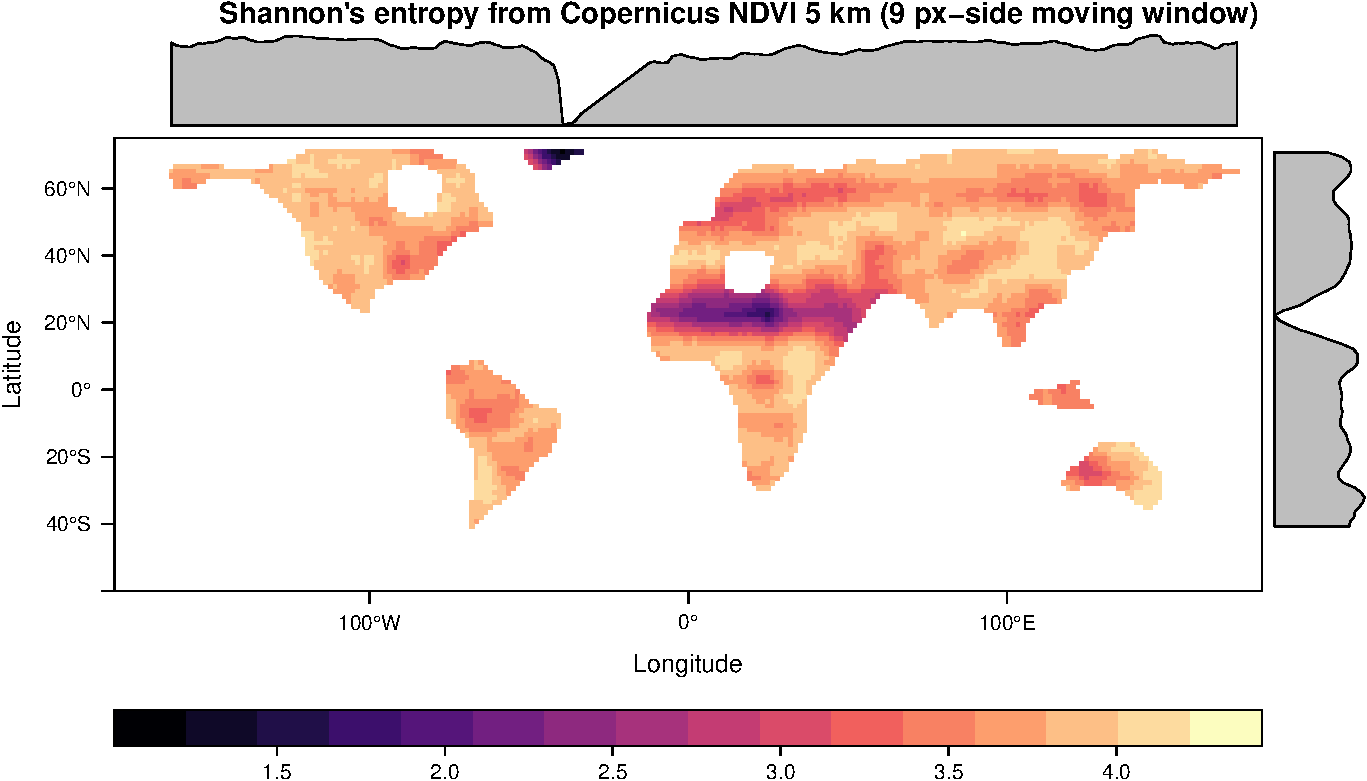
\includegraphics[width=0.95\linewidth]{vignettes_rasterdiv_files/figure-latex/fig02-1} \end{center}

\begin{Shaded}
\begin{Highlighting}[]
\CommentTok{#Pielou's Evenness}
\KeywordTok{levelplot}\NormalTok{(piera,}\DataTypeTok{main=}\StringTok{"Pielou's evenness from Copernicus NDVI 5 km (9 px-side moving window)"}\NormalTok{,}\DataTypeTok{as.table =}\NormalTok{ T,}\DataTypeTok{layout=}\KeywordTok{c}\NormalTok{(}\DecValTok{0}\NormalTok{,}\DecValTok{1}\NormalTok{,}\DecValTok{1}\NormalTok{), }\DataTypeTok{ylim=}\KeywordTok{c}\NormalTok{(}\OperatorTok{-}\DecValTok{60}\NormalTok{,}\DecValTok{75}\NormalTok{), }\DataTypeTok{margin =} \KeywordTok{list}\NormalTok{(}\DataTypeTok{draw =} \OtherTok{TRUE}\NormalTok{))}
\end{Highlighting}
\end{Shaded}

\begin{center}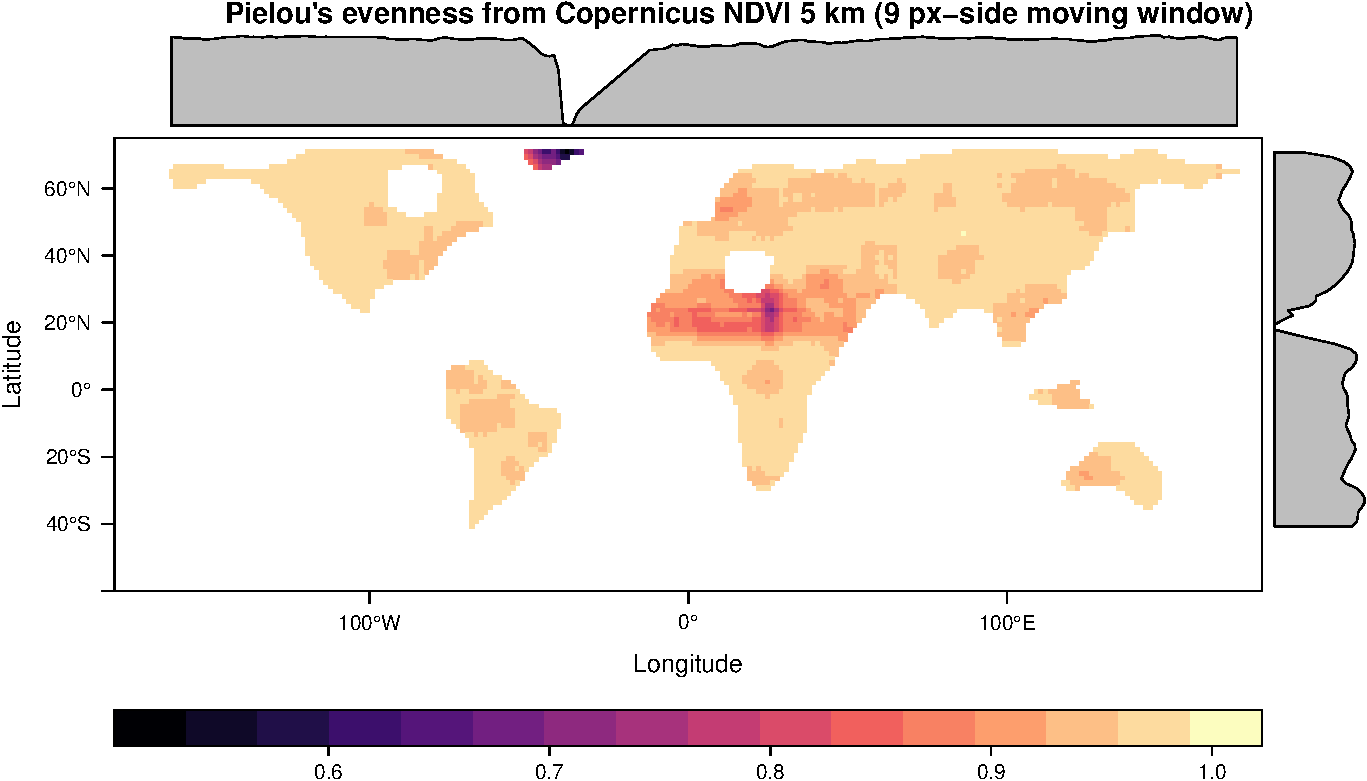
\includegraphics[width=0.95\linewidth]{vignettes_rasterdiv_files/figure-latex/fig03-1} \end{center}

\begin{Shaded}
\begin{Highlighting}[]
\CommentTok{#Berger-Parker' Index}
\KeywordTok{levelplot}\NormalTok{(berra,}\DataTypeTok{main=}\StringTok{"Berger-Parker's index from Copernicus NDVI 5 km (9 px-side moving window)"}\NormalTok{,}\DataTypeTok{as.table =}\NormalTok{ T,}\DataTypeTok{layout=}\KeywordTok{c}\NormalTok{(}\DecValTok{0}\NormalTok{,}\DecValTok{1}\NormalTok{,}\DecValTok{1}\NormalTok{), }\DataTypeTok{ylim=}\KeywordTok{c}\NormalTok{(}\OperatorTok{-}\DecValTok{60}\NormalTok{,}\DecValTok{75}\NormalTok{), }\DataTypeTok{margin =} \KeywordTok{list}\NormalTok{(}\DataTypeTok{draw =} \OtherTok{TRUE}\NormalTok{))}
\end{Highlighting}
\end{Shaded}

\begin{center}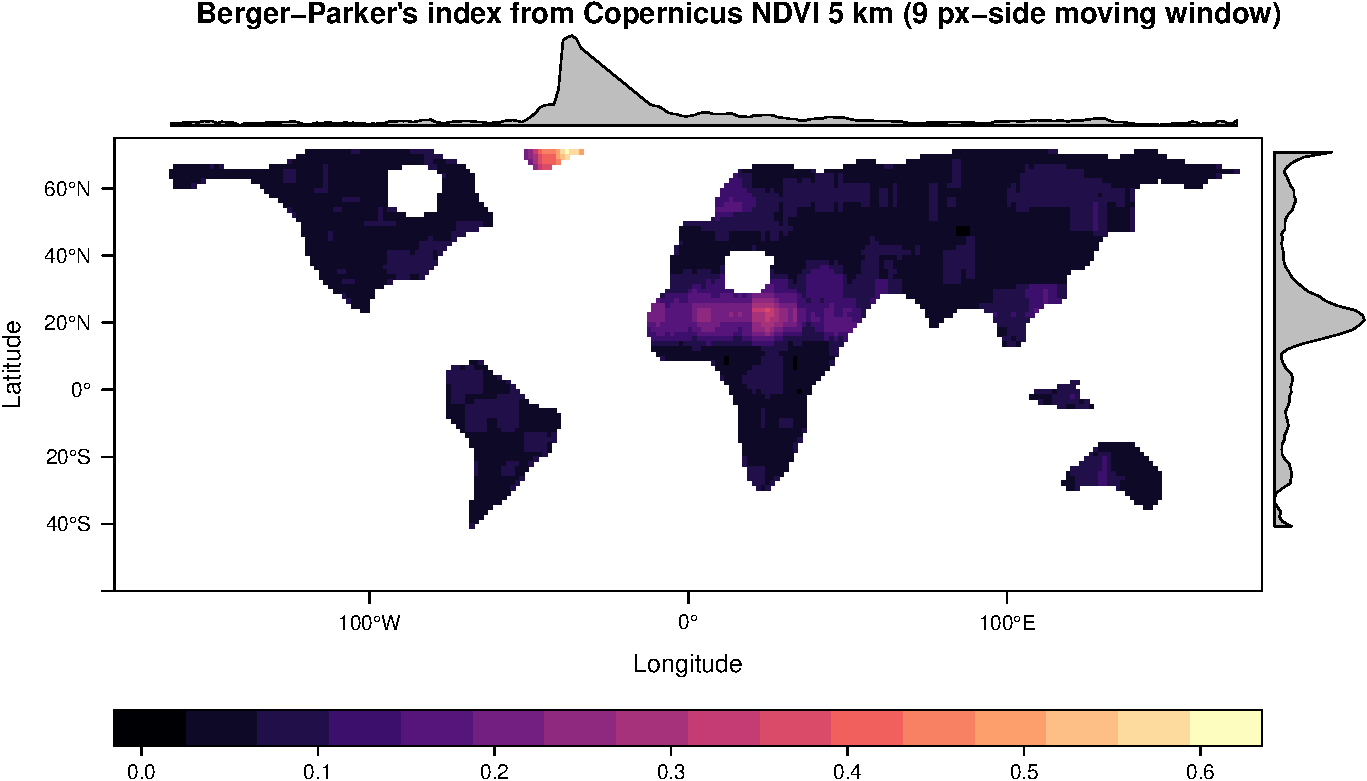
\includegraphics[width=0.95\linewidth]{vignettes_rasterdiv_files/figure-latex/fig04-1} \end{center}

\begin{Shaded}
\begin{Highlighting}[]
\CommentTok{#Rao's quadratic Entropy}
\KeywordTok{levelplot}\NormalTok{(crera,}\DataTypeTok{main=}\StringTok{"Rao's quadratic entropy from Copernicus NDVI 5 km (9 px-side moving window)"}\NormalTok{,}\DataTypeTok{as.table =}\NormalTok{ T,}\DataTypeTok{layout=}\KeywordTok{c}\NormalTok{(}\DecValTok{0}\NormalTok{,}\DecValTok{1}\NormalTok{,}\DecValTok{1}\NormalTok{), }\DataTypeTok{ylim=}\KeywordTok{c}\NormalTok{(}\OperatorTok{-}\DecValTok{60}\NormalTok{,}\DecValTok{75}\NormalTok{), }\DataTypeTok{margin =} \KeywordTok{list}\NormalTok{(}\DataTypeTok{draw =} \OtherTok{TRUE}\NormalTok{))}
\end{Highlighting}
\end{Shaded}

\begin{center}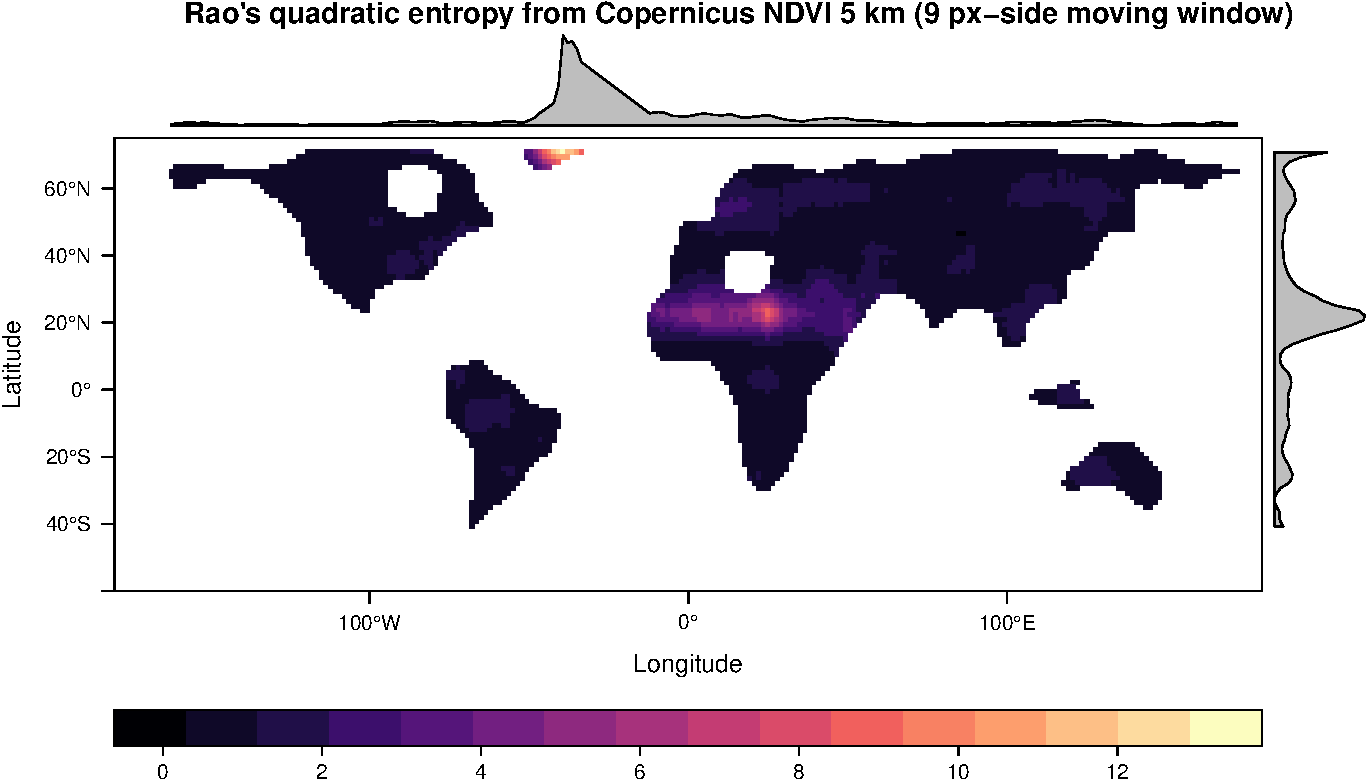
\includegraphics[width=0.95\linewidth]{vignettes_rasterdiv_files/figure-latex/fig05-1} \end{center}

\begin{Shaded}
\begin{Highlighting}[]
\CommentTok{#Cumulative Residual Entropy}
\KeywordTok{levelplot}\NormalTok{(crera,}\DataTypeTok{main=}\StringTok{"Cumulative Resiudal Entropy from Copernicus NDVI 5 km (9 px-side moving window)"}\NormalTok{,}\DataTypeTok{as.table =}\NormalTok{ T,}\DataTypeTok{layout=}\KeywordTok{c}\NormalTok{(}\DecValTok{0}\NormalTok{,}\DecValTok{1}\NormalTok{,}\DecValTok{1}\NormalTok{), }\DataTypeTok{ylim=}\KeywordTok{c}\NormalTok{(}\OperatorTok{-}\DecValTok{60}\NormalTok{,}\DecValTok{75}\NormalTok{), }\DataTypeTok{margin =} \KeywordTok{list}\NormalTok{(}\DataTypeTok{draw =} \OtherTok{TRUE}\NormalTok{))}
\end{Highlighting}
\end{Shaded}

\begin{center}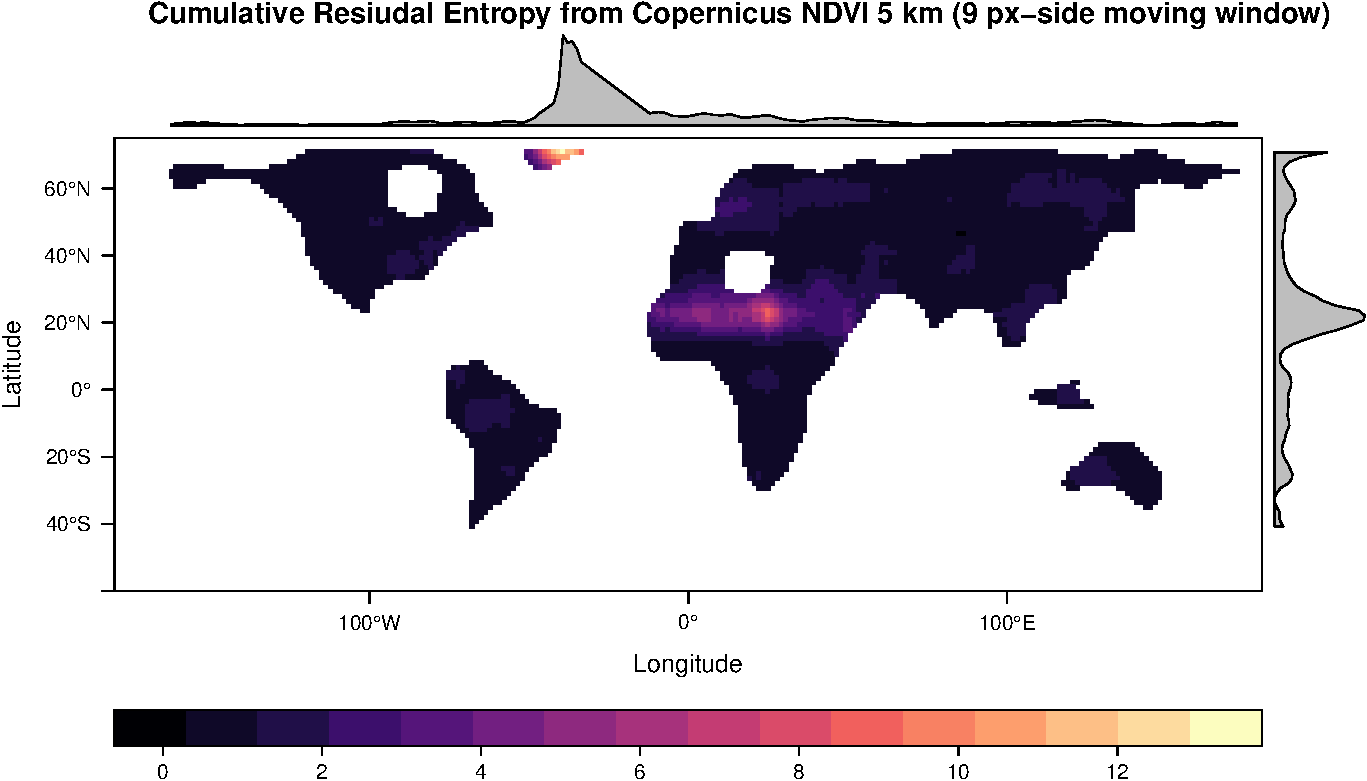
\includegraphics[width=0.95\linewidth]{vignettes_rasterdiv_files/figure-latex/fig06-1} \end{center}

\begin{Shaded}
\begin{Highlighting}[]
\CommentTok{#Hill's numbers (alpha=0, 1, 1.5 and 2)}
\KeywordTok{levelplot}\NormalTok{(}\KeywordTok{stack}\NormalTok{(hilra),}\DataTypeTok{main=}\StringTok{"Hill's numbers from Copernicus NDVI 5 km (9 px-side moving window)"}\NormalTok{,}\DataTypeTok{as.table =}\NormalTok{ T,}\DataTypeTok{layout=}\KeywordTok{c}\NormalTok{(}\DecValTok{0}\NormalTok{,}\DecValTok{5}\NormalTok{,}\DecValTok{1}\NormalTok{),}\DataTypeTok{names.attr=}\KeywordTok{paste}\NormalTok{(}\StringTok{"alpha"}\NormalTok{,}\KeywordTok{seq}\NormalTok{(}\DecValTok{0}\NormalTok{,}\DecValTok{2}\NormalTok{,}\FloatTok{0.5}\NormalTok{),}\DataTypeTok{sep=}\StringTok{" "}\NormalTok{), }\DataTypeTok{ylim=}\KeywordTok{c}\NormalTok{(}\OperatorTok{-}\DecValTok{60}\NormalTok{,}\DecValTok{75}\NormalTok{))}
\end{Highlighting}
\end{Shaded}

\begin{center}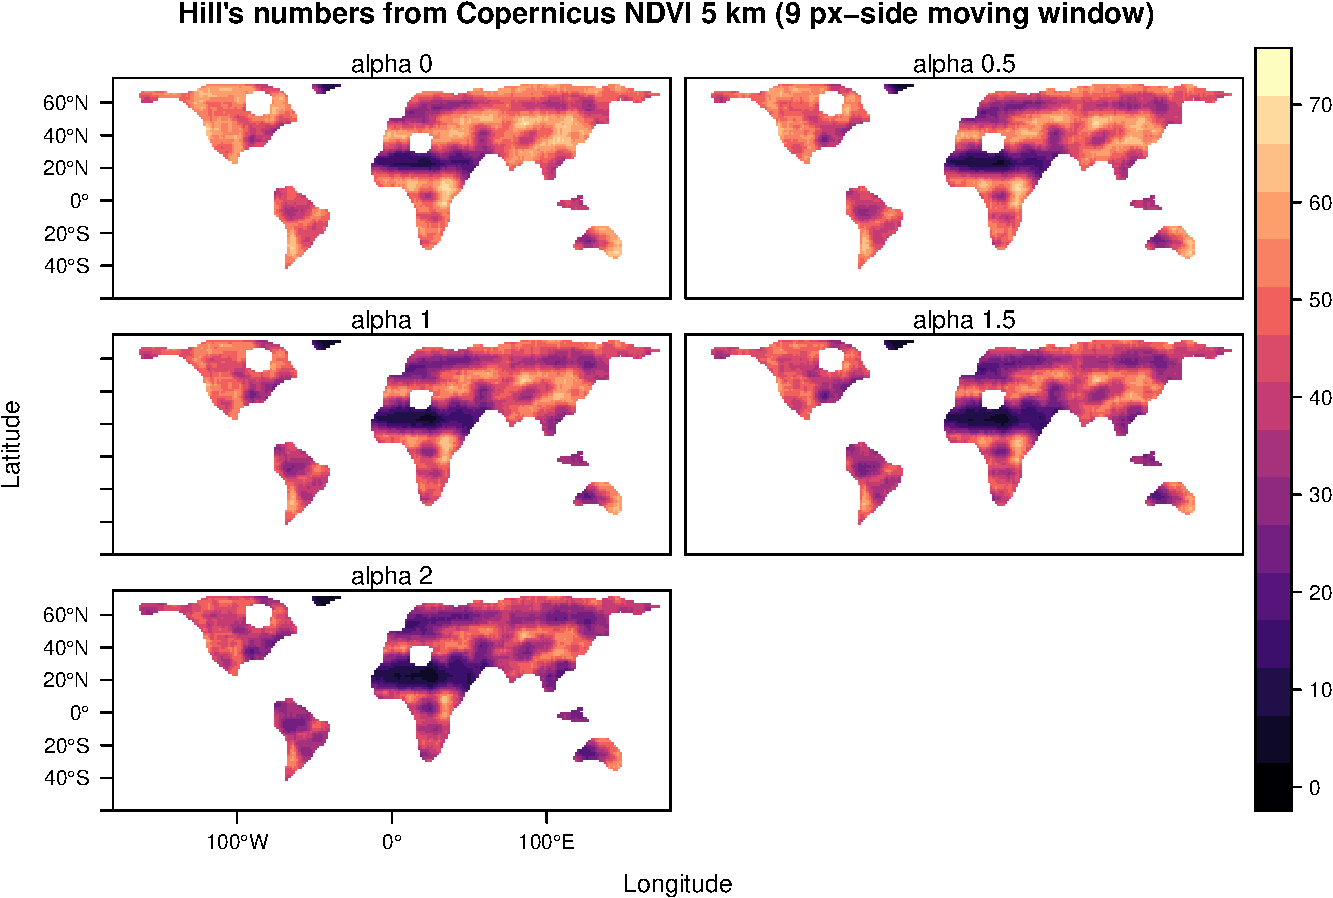
\includegraphics[width=0.95\linewidth]{vignettes_rasterdiv_files/figure-latex/fig07-1} \end{center}

\begin{Shaded}
\begin{Highlighting}[]
\CommentTok{#Renyi' Index (alpha=0, 1, 1.5 and 2)}
\KeywordTok{levelplot}\NormalTok{(}\KeywordTok{stack}\NormalTok{(renra),}\DataTypeTok{main=}\StringTok{"Renyi's entropy from Copernicus NDVI 5 km (9 px-side moving window)"}\NormalTok{,}\DataTypeTok{as.table =}\NormalTok{ T,}\DataTypeTok{layout=}\KeywordTok{c}\NormalTok{(}\DecValTok{0}\NormalTok{,}\DecValTok{5}\NormalTok{,}\DecValTok{1}\NormalTok{),}\DataTypeTok{names.attr=}\KeywordTok{paste}\NormalTok{(}\StringTok{"alpha"}\NormalTok{,}\KeywordTok{seq}\NormalTok{(}\DecValTok{0}\NormalTok{,}\DecValTok{2}\NormalTok{,}\FloatTok{0.5}\NormalTok{),}\DataTypeTok{sep=}\StringTok{" "}\NormalTok{), }\DataTypeTok{ylim=}\KeywordTok{c}\NormalTok{(}\OperatorTok{-}\DecValTok{60}\NormalTok{,}\DecValTok{75}\NormalTok{), }\DataTypeTok{margin =} \KeywordTok{list}\NormalTok{(}\DataTypeTok{draw =} \OtherTok{FALSE}\NormalTok{))}
\end{Highlighting}
\end{Shaded}

\begin{center}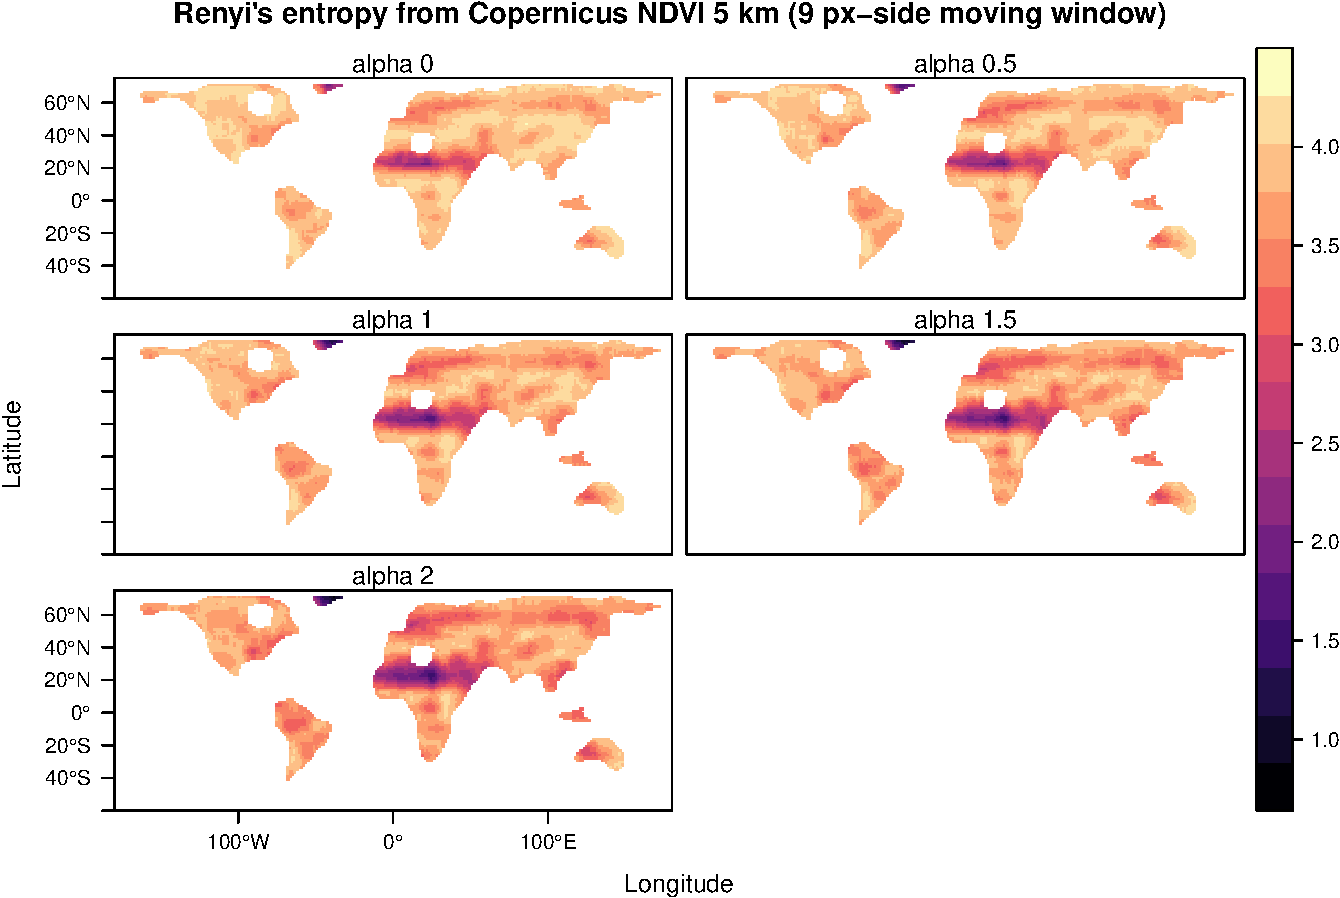
\includegraphics[width=0.95\linewidth]{vignettes_rasterdiv_files/figure-latex/fig08-1} \end{center}

\end{document}
